\begin{tcolorbox}
Show that the following limit does not exitst \[
\lim_{z\to0}\Big(\frac{\bar z}{z}\Big)^2
\] Do this by letting nonzero points $z=(x,0)$ and $z=(x,x)$ approach the origin. (Note that it is not sufficient to simply consider points $z=(x,0)$ and $z=(0,y)$.)
\end{tcolorbox}
\begin{proof}[\Sol]
	Let $z=x+iy\in\C$ with $x,y\in\mathbb{R}$. Then \[
	\left(\frac{\overline{z}}{z}\right)^{\!2}
	=\left(\frac{x-iy}{x+iy}\right)^{\!2}.
	\] If $z=re^{i\theta}$ with $r>0$, then $\bar z/z=e^{-2i\theta}$, so $|(\bar z/z)^2|=|e^{-4i\theta}|=1$.
	\begin{center}
		\begin{tikzpicture}[>=Latex,scale=1]
			% =============== z-plane (paths to the origin) ===============
			\begin{scope}
				% axes
				\draw[->] (-2.0,0) -- (2.0,0) node[right] {$\Re z$};
				\draw[->] (0,-2.0) -- (0,2.0) node[above] {$\Im z$};
				\node at (0,-2.25) {$z$-plane (approach $z\to 0$)};
				
				% origin as a hole (z=0 excluded)
				\fill[white] (0,0) circle (2.6pt);
				\draw[red] (0,0) circle (2pt) node[above right] {$z=0$ (undefined)};
				
				% Path 1: real axis y=0 (blue)
				\draw[blue!70,very thick,->] (-2,0) -- (-0.05,0) node[midway, above] {Path1: $y=0$};
				
				% Path 2: diagonal y=x (teal)
				\draw[teal!70,very thick,->] (-1.75,-1.75) -- (-0.05,-0.05) node[midway, xshift=-1.25cm] {Path2: $y=x$};
			\end{scope}
			% =============== mapping arrow ===============
			\draw[->,thick] (3.5,0) -- (6,0)
			node[midway,above] {$f(z)=\left(\dfrac{\overline z}{z}\right)^2$};
			% =============== value plane (outputs) ===============
			\begin{scope}[xshift=8.4cm]
				% axes
				\draw[->] (-2,0) -- (2,0) node[below right] {$\Re$};
				\draw[->] (0,-1.8) -- (0,1.8) node[left] {$\Im$};
				\node at (0,-2.05) {value plane of $f(z)$};
				
				% unit circle (context): |(\bar z/z)^2| = 1 for z≠0
				\draw[gray!40] (0,0) circle (1);
				
				% images of the two paths (constants 1 and -1)
				% Path 1 (y=0) -> 1
				\fill[blue!70] (1,0) circle (2.4pt) node[above right] {$1$};
				\draw[blue!70,->] (1.1,.75) to[bend left=10] (1,0);
				\node[blue!70,align=center] at (1,1.2)
				{along $y=0$:\\ $f(z)\equiv 1$};
				
				% Path 2 (y=x) -> -1
				\fill[teal!70] (-1,0) circle (2.4pt) node[below left] {$-1$};
				\draw[teal!70,->] (-1.1,-0.75) to[bend left=10] (-1,0);
				\node[teal!70,align=center] at (-1,-1.2)
				{along $y=x$:\\ $f(z)\equiv -1$};
				
				%	% conclusion box
				%	\node[draw,rounded corners=2pt,align=left,anchor=north] at (0,-1.25)
				%	{$\displaystyle \lim_{z\to 0}\left(\frac{\overline z}{z}\right)^2\ \text{does not exist},$\\
					%		since the limits along $y=0$ and $y=x$ differ.};
			\end{scope}
		\end{tikzpicture}
	\end{center}
	\medskip
	\noindent\textbf{(1) Path 1: approach along the real axis $y=0$}
	
	Let $z=x+0i=x$ with $x\in\mathbb{R}\setminus\{0\}$ and $x\to 0$. Then $
	\displaystyle\left(\frac{\overline{z}}{z}\right)^2
	=\left(\frac{x}{x}\right)^2
	=1$.
	
	\medskip
	\noindent\textbf{(2) Path 2: approach along the diagonal $y=x$}
	
	Let $z=x+ix=(1+i)x$ with $x\in\mathbb{R}\setminus\{0\}$ and $x\to 0$. Then
	\[
	\frac{\overline{z}}{z}
	=\frac{\overline{(1+i)x}}{(1+i)x}
	=\frac{(1-i)\,x}{(1+i)\,x}
	=\frac{1-i}{1+i}
	=\frac{(1-i)^2}{(1+i)(1-i)}
	=\frac{1-2i+i^2}{1- i^2}
	=\frac{1-2i-1}{2}
	=\frac{-2i}{2}
	=-i.
	\]
	Hence
	\[
	\left(\frac{\overline{z}}{z}\right)^2
	=(-i)^2
	=-1.
	\] 
	
	\medskip
	\noindent\textbf{(3) Conclusion}
	
	Since the limits along these two paths are different (namely $1$ and $-1$), the limit cannot exist.
\end{proof}

\begin{tcolorbox}
Let \[
f(z)=\begin{cases} \bar z^2/z,& z\neq0,\\ 0,& z=0.\end{cases}
\] Show that if $z=0$, then $\Delta w/\Delta z=1$ at eatch nonzero point on the real and imaginary axes in the $\Delta z$, or $\Delta x\Delta y$, plane. Then show that $\Delta w/\Delta z=-1$ at each nonzero point $(\Delta x, \Delta y)$ on the line $\Delta y=\Delta x$ in that plane. Conclude from these observations that $f'(0)$ does not exist. Note that to obtain this result, it is not sufficient to consider only horizontal and vertical approaches to the origin in the $\Delta z$ plane.
\end{tcolorbox}
\begin{proof}
	Let $\frac{\Delta w}{\Delta z}
	=\frac{f(\Delta z)-f(0)}{\Delta z}
	\quad(\Delta z\neq 0)$. Since $f(0)=0$, for $\Delta z\neq0$, $\displaystyle
	\frac{\Delta w}{\Delta z}
	=\frac{f(\Delta z)}{\Delta z}
	=\frac{\overline{\Delta z}^{\,2}}{(\Delta z)^2}$.
	
	\medskip
	\noindent\textbf{(1) Real and imaginary axes.}
	\begin{itemize}
		\item Real axis: $\Delta z=x$ with $x\in\mathbb{R}\setminus\{0\}$, $\displaystyle
		\frac{\Delta w}{\Delta z}=\frac{\overline{x}^{\,2}}{x^2}=\frac{x^2}{x^2}=1$.
		\begin{center}
			\begin{tikzpicture}[>=Latex,scale=1.05]	
				%================ z-plane: explicit paths =================
				\begin{scope}
					% axes
					\draw[->] (-2,0) -- (2,0) node[right] {$\Re z$};
					\draw[->] (0,-2) -- (0,2) node[above] {$\Im z$};
					% hole at the origin (Delta z = 0 excluded)
					\fill[white] (0,0) circle (2.6pt);
					\draw[red] (0,0) circle (2pt) node[above right] {$\Delta z=0$ (excluded)};
					% Path A: real axis, Δz = x, x→0, x≠0
					\draw[line width=1.6pt,blue!70,->] (-2.8,0) -- (-0.12,0);
					\draw[line width=1.6pt,blue!70,->] ( 2.8,0) -- ( 0.12,0);
					\node[blue!70,anchor=north] at (0,-0.10)
					{$\displaystyle \text{Path A: }\Delta z=x,\ x\in\mathbb R\!\setminus\!\{0\},\ x\to 0$};
				\end{scope}
				%================ mapping arrow =================
				\draw[->,thick] (3.5,0) -- (7,0)
				node[midway,above] {$\displaystyle \frac{\Delta w}{\Delta z}=\frac{\overline{\Delta z}^{\,2}}{(\Delta z)^2}$};
				%================ value plane: constant images =================
				\begin{scope}[xshift=9.4cm]
					% axes
					\draw[->] (-2,0) -- (2,0) node[right] {$\Re f(z)$};
					\draw[->] (0,-2) -- (0,2) node[above] {$\Im f(z)$};
					%	\node at (0,-2.55) {$f(z)$-plane of $\Delta w/\Delta z$};
					% unit circle for context (|Δw/Δz|=1 for Δz≠0)
					\draw[gray!35] (0,0) circle (1);
					% Image of Path A (real axis): constant 1
					\fill[blue!70] (1,0) circle (2.6pt) node[above right] {$\displaystyle \text{Path A: } \frac{\overline{x}^{\,2}}{x^2}=1$};
				\end{scope}
			\end{tikzpicture}
		\end{center}
		\item Imaginary axis: $\Delta z=iy$ with $y\in\mathbb{R}\setminus\{0\}$, $\displaystyle
		\frac{\Delta w}{\Delta z}
		=\frac{\overline{iy}^{\,2}}{(iy)^2}
		=\frac{(-iy)^2}{(iy)^2}
		=\frac{-y^2}{-y^2}=1$.
		\begin{center}
			\begin{tikzpicture}[>=Latex,scale=1.05]	
				%================ z-plane: explicit paths =================
				\begin{scope}
					% axes
					\draw[->] (-2,0) -- (2,0) node[right] {$\Re z$};
					\draw[->] (0,-2) -- (0,2) node[above] {$\Im z$};
					% hole at the origin (Delta z = 0 excluded)
					\fill[white] (0,0) circle (2.6pt);
					\draw[red] (0,0) circle (2pt) node[above right] {$\Delta z=0$ (excluded)};
					% Path B: imaginary axis, Δz = iy, y→0, y≠0
					\draw[line width=1.6pt,purple!70,->] (0,-2.0) -- (0,-0.12);
					\draw[line width=1.6pt,purple!70,->] (0, 2.0) -- (0, 0.12);
					\node[purple!70,anchor=north] at (0,-2)
					{$\displaystyle \text{Path B: }\Delta z=iy,\ y\in\mathbb R\!\setminus\!\{0\},\ y\to 0$};
				\end{scope}
				%================ mapping arrow =================
				\draw[->,thick] (3.5,0) -- (7,0)
				node[midway,above] {$\displaystyle \frac{\Delta w}{\Delta z}=\frac{\overline{\Delta z}^{\,2}}{(\Delta z)^2}$};
				%================ value plane: constant images =================
				\begin{scope}[xshift=9.4cm]
					% axes
					\draw[->] (-2,0) -- (2,0) node[right] {$\Re f(z)$};
					\draw[->] (0,-2) -- (0,2) node[above] {$\Im f(z)$};
					%	\node at (0,-2.55) {$f(z)$-plane of $\Delta w/\Delta z$};
					% unit circle for context (|Δw/Δz|=1 for Δz≠0)
					\draw[gray!35] (0,0) circle (1);
					% Image of Path B (imag axis): constant 1
					\fill[purple!70] (1,0) circle (2.6pt);
					\node[purple!70,anchor=north west] at (0.95,-0.18)
					{$\displaystyle \text{Path B: } \frac{\overline{(iy)}^{\,2}}{(iy)^2}=1$};
				\end{scope}
			\end{tikzpicture}
		\end{center}
	\end{itemize}
	
	\noindent\textbf{(2) Line $\Delta y=\Delta x$.}
	Let $\Delta z=(1+i)x$ with $x\in\mathbb{R}\setminus\{0\}$. Then
	\[
	\frac{\Delta w}{\Delta z}
	=\frac{\overline{(1+i)x}^{\,2}}{((1+i)x)^2}
	=\frac{((1-i)x)^2}{((1+i)x)^2}
	=\frac{(1-i)^2}{(1+i)^2}
	=\frac{-2i}{2i}=-1.
	\]
	\begin{center}
		\begin{tikzpicture}[>=Latex,scale=1.05]	
			%================ z-plane: explicit paths =================
			\begin{scope}
				% axes
				\draw[->] (-2,0) -- (2,0) node[right] {$\Re z$};
				\draw[->] (0,-2) -- (0,2) node[above] {$\Im z$};
				%	\node at (0,-2.55) {$z$-plane (approach $\Delta z\to 0$)$\,$};	
				% hole at the origin (Delta z = 0 excluded)
				\fill[white] (0,0) circle (2.6pt);
				\draw[red] (0,0) circle (2pt) node[above right] {$\Delta z=0$ (excluded)};
				% Path C: diagonal Δy=Δx, i.e., Δz = (1+i)t, t→0, t≠0
				\draw[line width=1.6pt,teal!75,->] (-2.2,-2.2) -- (-0.12,-0.12);
				\draw[line width=1.6pt,teal!75,->] ( 2.2, 2.2) -- ( 0.12, 0.12);
				\node[teal!75,anchor=south east] at (5,-2.35)
				{$\displaystyle \text{Path C: }\Delta z=(1+i)t,\ t\in\mathbb R\!\setminus\!\{0\},\ t\to 0$};
			\end{scope}
			%================ mapping arrow =================
			\draw[->,thick] (3.5,0) -- (7,0)
			node[midway,above] {$\displaystyle 
				\frac{\Delta w}{\Delta z}=\frac{\overline{\Delta z}^{\,2}}{(\Delta z)^2}
				%	\displaystyle \,f(z)=\begin{cases}
					%		\overline z^{\,2}/z &\text{if}\; z\neq 0\\
					%		0 &\text{if}\; z=0
					%	\end{cases}
				$};
			%================ value plane: constant images =================
			\begin{scope}[xshift=9.4cm]
				% axes
				\draw[->] (-2,0) -- (2,0) node[right] {$\Re f(z)$};
				\draw[->] (0,-2) -- (0,2) node[above] {$\Im f(z)$};
				%	\node at (0,-2.55) {$f(z)$-plane of $\Delta w/\Delta z$};
				% Image of Path C (diagonal): constant -1
				\fill[teal!75] (-1,0) circle (2.6pt) node[below] {$\displaystyle \text{Path C: } \frac{\overline{(1+i)t}^{\,2}}{((1+i)t)^2}=-1$};
			\end{scope}
		\end{tikzpicture}
	\end{center}
	\medskip
	\noindent\textbf{(3) Conclusion.}
	Since the difference quotient equals $1$ along the axes but $-1$ along the line $\Delta y=\Delta x$, the limit
	\[
	\lim_{\Delta z\to 0}\frac{f(\Delta z)-f(0)}{\Delta z}
	\]
	depends on the path and therefore does not exist. Consequently, $f'(0)$ does not exist.
\end{proof}	
\vfill
\begin{tcolorbox}
Let \[
f(z)=\bar z,\quad f(z)=2x+ixy^2,\quad f(z)=e^{\bar z}
\] Then show that $f'(z)$ does not exists at any point.
\end{tcolorbox}
\begin{proof}[\Sol]
	Let \(z=x+iy\) and \(f(z)=u+iv\) with $x,y,u,v\in\R$. The Cauchy--Riemann equations \[
	u_x=v_y,\qquad u_y=-\,v_x
	\]
	are necessary and sufficient for complex differentiability.
	
	\medskip
	\noindent\textbf{(1) \(f_1(z)=\overline z=\overline{x+iy}=x-iy\).}
	
	Here \(u(x,y)=x,\ v(x,y)=-y\). Thus \[
	u_x=1,\quad u_y=0,\quad v_x=0,\quad v_y=-1.
	\]
	The CR require \(u_x=v_y\), i.e.\ \(1=-1\), which is impossible. Hence \(f_1'\) does not exist anywhere.
	
	\medskip\newpage
	\noindent\textbf{(2) \(f_2(z)=2x+i\,x y^{2}\).}
	
	Here \(u(x,y)=2x,\ v(x,y)=x y^{2}\). Thus
	\[
	u_x=2,\quad u_y=0,\quad v_x=y^{2},\quad v_y=2xy.
	\]
	The CR demand \[
	\begin{cases} u_x=v_y\\ u_y=-v_x \end{cases}\implies
	\begin{cases} 2=2xy\\ 0=y^2 \end{cases}\implies
	\begin{cases} xy=1\\ y=0 \end{cases}.
	\] These cannot hold simultaneously for any \(x\). Hence CR fail at every point, so \(f_2'\) exists nowhere.
	
	\medskip
	\noindent\textbf{(3) \(f_3(z)=e^{\overline z}\).}
	
	Let \(\overline z=x-iy\). Then $f_3(x,y)=e^{x-iy}=e^{x}(\cos y-i\sin y)$, so \[
	u(x,y)=e^{x}\cos y,\qquad v(x,y)=-\,e^{x}\sin y.
	\] Compute \[
	u_x=e^{x}\cos y,\quad u_y=-e^{x}\sin y,\quad
	v_x=-e^{x}\sin y,\quad v_y=-e^{x}\cos y.
	\] The CR give \[
	\begin{cases} u_x=v_y\\ u_y=-v_x \end{cases}\implies
	\begin{cases} e^x\cos y=-e^x\cos y\\ -e^x\sin y=+e^x\sin y \end{cases}\implies
	\begin{cases} \cos y = 0\\ \sin y=0 \end{cases}.
	\] These cannot hold simultaneously for any \(y\). Hence CR fail everywhere and \(f_3'\) exists nowhere.
\end{proof}

\vfill
\begin{tcolorbox}
Show that the function \[
f(z)=\ln r+i\theta\quad (r>0,\; 0<\theta<2\pi)
\] is analytic in the indicated domain of definition, with derivative $f'(z)=1/z$. Then show that th e composite function $g(z)=f(z^2+1)$ is analytic in the quadratic $x>0,y>0$ with derivative \[
g'(z)=\frac{2z}{z^2+1}.
\] (Suggestion: Observe that $\Im(z^2+1)>0$ when $x>0, y>0$)
\end{tcolorbox}
\begin{proof}[\sol]
	Let $z=x+iy=re^{i\theta}$ with $r=\sqrt{x^2+y^2}>0$ and $0<\theta<2\pi$. Define
	\[
	f(z)=\ln r+i\theta .
	\]
	Then $f$ is analytic on the slit plane
	\begin{center}
		\begin{minipage}{.475\textwidth} \[
			\Omega:=\{\,z\in\mathbb{C}: r>0,\ 0<\theta<2\pi\,\}=\mathbb{C}\setminus[0,\infty),
			\] and $f'(z)=\frac{1}{z}\; (z\in\Omega)$.
		\end{minipage}\hfill
		\begin{minipage}{.475\textwidth}\centering
			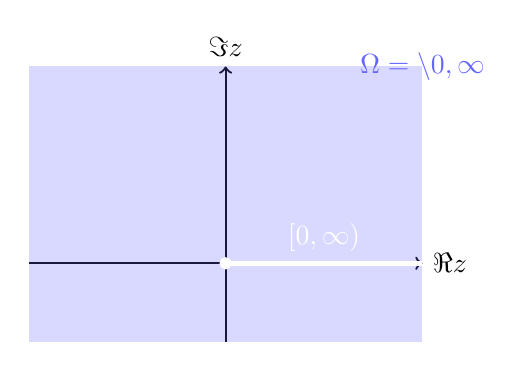
\begin{tikzpicture}
				% axes
				\draw[->, thick] (-2.5,0) -- (2.5,0) node[right] {$\Re z$};
				\draw[->, thick] (0,-1) -- (0,2.5) node[above] {$\Im z$};
				% shade domain
				\fill[blue!60, opacity=.25] (-2.5,-1) rectangle (2.5,2.5);
				\node[blue!60] at (2.5,2.5) {$\Omega=\C\setminus\intco{0,\infty}$};
				% slit: [0, +∞) on real axis
				\filldraw[white] (0,0) circle (2pt);
				\draw[white,ultra thick] (0,0) -- (2.5,0) node[midway, above] {$[0,\infty)$};
			\end{tikzpicture}
		\end{minipage}
	\end{center}
	Write $f=u+iv$ with \[
	u(x,y)=\ln r=\frac12\ln(x^2+y^2),\qquad v(x,y)=\theta=\Arg(z)\in(0,2\pi).
	\]
	On $\Omega$ the functions $u,v$ are $C^1$ and their partials are:
	\[
	u_x=\frac{x}{x^2+y^2},\quad u_y=\frac{y}{x^2+y^2},\qquad
	v_x=-\frac{y}{x^2+y^2},\quad v_y=\frac{x}{x^2+y^2}.
	\]
	Hence the Cauchy--Riemann equations hold on $\Omega$:
	\[
	u_x=v_y=\frac{x}{x^2+y^2},\qquad u_y=-v_x=\frac{y}{x^2+y^2}.
	\]
	Since these partials are continuous on $\Omega$, $f$ is analytic there. Its complex derivative is
	\[
	f'(z)=u_x+iv_x=\frac{x}{x^2+y^2}+i\!\left(-\frac{y}{x^2+y^2}\right)
	=\frac{x-iy}{x^2+y^2}=\frac{1}{x+iy}=\frac{1}{z}.
	\]
	For $g(z)=f(z^2+1)$, compute
	\begin{align*}
		z^2+1&=(x+iy)^2+1\\
		&=(x^2-y^2+2ixy) +1 \\
		&=(x^2-y^2+1)+i(2xy).
	\end{align*}
	If $x>0$ and $y>0$, then $\Im(z^2+1)=2xy>0$, so $z^2+1$ lies in the open upper half-plane $\mathbb{H}$, in particular in $\Omega$ (its argument lies in $(0,\pi)\subset(0,2\pi)$). Thus $g$ is the composition of analytic functions on the first quadrant $Q_1$, hence analytic on $Q_1$. By the chain rule, \[
	g'(z)=f'(z^2+1)\cdot(2z)=\frac{2z}{z^2+1}\qquad (z\in Q_1).
	\]
\end{proof}
